%==============================================================================
% Final Project Report -- Parallel Programming, Spring 2026
% Self-contained Overleaf package root: report/
% Required plot assets are in: paper_assets/
%==============================================================================
\documentclass[conference]{IEEEtran}
\IEEEoverridecommandlockouts

\usepackage{cite}
\usepackage{amsmath,amssymb,amsfonts}
\usepackage{array}
\usepackage{booktabs}
\usepackage{graphicx}
\usepackage{textcomp}
\usepackage{xcolor}
\usepackage{listings}
\usepackage{url}
\usepackage{float}
\usepackage{placeins}
\usepackage[hidelinks]{hyperref}

\graphicspath{{paper_assets/}}

\newcommand{\mainbodyendpage}{?}
\AtEndDocument{%
  \typeout{====================================================}%
  \typeout{[PAGE BUDGET] Main body + references end on page \mainbodyendpage\space (limit: 6, Appendix excluded).}%
  \typeout{====================================================}%
}

\lstset{
  basicstyle=\ttfamily\scriptsize,
  breaklines=true,
  frame=single,
  columns=fullflexible,
  showstringspaces=false,
  keepspaces=true,
  xleftmargin=0.2em,
  aboveskip=0.35em,
  belowskip=0.35em
}

\begin{document}

\title{Does Claude Optimize for the First Step?\\[0.1ex]
{\large\textbf{Measuring Short-Horizon Preference in LLM-Guided GPU Kernel Optimization}}\\[0.1ex]
{\normalsize Final Project --- Parallel Programming, Spring 2026}\vspace{0.1ex}}

\author{%
\IEEEauthorblockN{\textbf{Kuan-Lei Wu}}
\IEEEauthorblockA{R14944049 \\
GINM \\
r14944049@ntu.edu.tw}
\and
\IEEEauthorblockN{\textbf{Sheng Chen}}
\IEEEauthorblockA{R11922119 \\
CSIE \\
r11922119@ntu.edu.tw}
\and
\IEEEauthorblockN{\textbf{Young Lee}}
\IEEEauthorblockA{R14942037 \\
GICE \\
r14942037@ntu.edu.tw}%
}

\maketitle

\begin{abstract}
GPU kernel optimization is path-dependent: a first edit can produce a quick
speedup and then plateau, while a weaker first edit may open a better
trajectory. This report studies whether Claude's first-move preference reflects
immediate speedup or the best speedup found after continuing optimization. For
four HecBench CUDA kernels, Claude generated and ranked five candidate
optimization plans under either a default prompt or an explicit long-horizon
prompt. Each plan was executed independently by a Worker branch for a fixed
budget of seven successful correctness-checked iterations. Using a
geomean-normalized rank-step penalty, the default prompt showed a small
iteration-1 penalty of 3.0\% per lower agent-ranking position but essentially
no final-speedup penalty, 0.0\%. The long-horizon prompt kept similar
iteration-1 alignment, 2.9\%, but raised final-speedup alignment to 11.2\%.
It also reduced top-choice final-speedup regret from 26.1\% to 10.8\%. The
logs show why prompting helps but is insufficient: Claude still exhibits
salient-metric fixation, wrong mechanism selection, algorithmic elegance bias,
and resource-tradeoff misses.
\end{abstract}

\begin{IEEEkeywords}
GPU optimization, CUDA, LLM agents, prompt engineering, performance analysis,
rank-step penalty
\end{IEEEkeywords}

\vspace{0.5em}
\noindent\fbox{\parbox{0.97\columnwidth}{\textbf{Project Category:}\quad
$\square$~\textbf{A} (Self-chosen topic)\qquad
$\boxtimes$~\textbf{B} (AI-agent code optimization)}}

\section{Introduction}

Large language model (LLM) coding agents are increasingly used as practical
optimization assistants. A simple workflow is attractive: give the agent a
kernel, ask it to optimize, run the benchmark, and repeat. The risk is that
kernel optimization is not a sequence of independent local edits. A CUDA
change that improves the first run can consume registers, reduce occupancy,
add shared-memory pressure, or fix only an easy local symptom. Another
direction may start slowly but create more room for later changes.

This report asks whether Claude's first-move preference is aligned with
short-term payoff, longer-horizon speedup, or neither. To measure that
preference, Claude is asked to generate and rank five candidate optimization
plans. This generate-and-rank step is a measurement probe rather than a normal
user interface: it exposes which starting directions Claude prefers before any
implementation outcomes are known. Each plan is then run independently by a
Worker branch under the same correctness and iteration budget.

The experiment also asks whether this preference changes when trajectory value
is stated explicitly. In a default prompt, Claude ranks plans by what it would
try first. In a long-horizon prompt, Claude is told that each plan will be
executed by a separate Worker for a fixed budget and is asked to rank plans by
which starting direction is most likely to reach the highest speedup within
that budget. The target is not the number seven itself; seven successful
iterations are simply the controlled search budget used to approximate
continuing optimization.

The contribution is not a new CUDA optimization technique. The contribution is
a controlled analysis of LLM-guided optimization behavior. I compare the two
prompt conditions, use magnitude-aware metrics instead of pure rank agreement,
and connect the numerical results to Worker logs. The main finding is that
Claude's default ranking weakly predicts which plan works immediately, but
almost does not predict which direction reaches the best speedup after the
optimization budget. Long-horizon prompting improves this alignment and
reduces regret, but the logs show persistent causal reasoning errors over
profiler signals and GPU resource tradeoffs.

\section{Background}

\subsection{Kernels and Optimization Angles}

The experiment uses CUDA kernels from HecBench, a heterogeneous-computing
benchmark suite with GPU implementations of common algorithms and application
kernels~\cite{hecbench}. I use four kernels whose optimization behavior is
understandable from code and profiler evidence, while still offering multiple
plausible optimization angles. This selection supports interpretable
trajectory analysis rather than broad benchmark coverage.

\begin{table}[t]
\centering
\caption{Kernels and optimization angles.}
\label{tab:kernels}
\scriptsize
\setlength{\tabcolsep}{2.5pt}
\begin{tabular}{@{}p{0.19\columnwidth}p{0.34\columnwidth}p{0.37\columnwidth}@{}}
\toprule
\textbf{Kernel} & \textbf{Main tension} & \textbf{Plausible angles} \\
\midrule
bitonic-sort & Mapping a sorting network onto GPU threads. &
Shared memory, global-memory layout, divergence, launch structure. \\
histogram & Parallelism versus atomic contention. &
Grid shape, pass fusion, allocation traffic, memory layout. \\
softmax & Memory latency versus memory traffic. &
Read reduction, occupancy, block size, latency hiding. \\
stencil3d & Bandwidth, precision, and tiling interact. &
Precision, coalescing, block shape, shared-memory tiling. \\
\bottomrule
\end{tabular}
\end{table}

\subsection{Why First Direction Matters}

CUDA performance constraints are coupled. Shared memory may reduce global
traffic but lower occupancy. Register-heavy rewrites may remove memory
operations but cause spilling. Changing precision can reduce bandwidth pressure
and also enable larger tiles. Grid size can reduce launch or pass overhead but
increase atomic contention. These tradeoffs mean the first edit is not merely a
local patch; it selects a region of the optimization landscape.

This coupling makes LLM-guided optimization interesting. An agent can know
many plausible CUDA tactics, but the valuable behavior is choosing a first
direction whose later refinements have headroom. The paper therefore measures
both iteration-1 speedup and the best speedup found after a fixed optimization
budget. The first is the payoff a naive loop sees immediately. The second is
closer to the goal of this line of work: finding a strong kernel implementation.

\section{Methodology}

\subsection{Agent Ranking Probe and Worker Execution}

For each kernel and prompt condition, Claude generated five candidate
optimization plans and ordered them from P1 to P5. I call this order the
\emph{agent ranking}. This ranking is not intended to model a normal user
interface; it is a probe for Claude's preference before outcome feedback. Each
ranked plan was assigned to an independent Worker branch. The Worker received
only that plan, edited an allowlisted source-file set, and repeatedly ran
\texttt{./src/run.sh}. A successful iteration means the run finished and
\texttt{out/latest\_run.json} reported \texttt{status: correct}. Compile
errors, correctness failures, profiling infrastructure errors, and
iteration-limit events were logged but did not count toward the seven
successful iterations.

This separation is important. If one Claude session repeatedly optimized a
kernel, later decisions would be affected by earlier outcomes. Here, the
generate-and-rank step is measured before any Worker sees a result. The five
branches start from the same baseline and are evaluated under the same rules,
so differences between branches can be interpreted as differences between
starting directions and the Worker trajectories they enable.

\subsection{Prompt Conditions}

Condition A used a default optimization prompt. Claude was asked to propose
exactly five distinct plans and rank them from highest to lowest priority based
on what it would try first to improve performance. The prompt did not mention
downstream Workers, the seven-iteration budget, or trajectory evaluation.

Condition B used a long-horizon prompt. Claude was told that a separate Worker
would execute each ranked plan for exactly seven iterations. It was asked to
rank plans by which starting direction was most likely to achieve the highest
peak speedup at any point within those iterations, considering how the first
direction opens or blocks later optimizations. Both conditions used the same
kernel sources, benchmark harness, correctness rule, Worker loop, and speedup
measurement. The intended independent variable is the horizon framing of the
plan ranking.

\subsection{Magnitude-Aware Metrics}

Pure rank metrics are too coarse for this question because they treat near ties
and large losses equally. I instead use a magnitude-aware rank-step penalty.
For one fixed kernel, prompt condition, and evaluation horizon, let $s_p$ be
the speedup of the plan at ranking position $p\in\{1,\ldots,5\}$. I first
divide each speedup by the geometric mean of the five plans:
\begin{equation}
g=\left(\prod_{p=1}^{5}s_p\right)^{1/5}, \qquad y_p=\frac{s_p}{g}.
\end{equation}
Thus $y_p=1$ means average for that kernel, $y_p=1.10$ means 10\% above that
kernel's typical plan, and $y_p=0.90$ means 10\% below it. After this
normalization, I pool the points for a condition and horizon and fit a straight
line from P1 to P5:
\begin{equation}
y_p = a + bp + \epsilon_p .
\end{equation}
The reported rank-step penalty is $-100b$. If the penalty is 3\%, then moving
one position lower in Claude's ranking corresponds to about 3\% lower speedup
relative to that kernel's typical branch. Positive means the ranking predicts
speedup; zero means it does not; negative means it is inverted.

I use this penalty at two horizons: iteration 1 and best speedup after the
fixed Worker budget. The \emph{greediness score} is the iteration-1 penalty
minus the final-speedup penalty. Positive greediness means the ranking is more
aligned with immediate gain; negative greediness means it is more aligned with
longer-horizon gain. Finally, I report top-choice regret:
\begin{equation}
R=\frac{s_{\mathrm{best}}-s_1}{s_{\mathrm{best}}}.
\end{equation}
This regret metric estimates the cost of following Claude's first-ranked plan
instead of exploring all five starting directions.

\section{Experimental Setup}

The design creates 40 Worker branches: four kernels, two prompt conditions, and
five ranked plans per condition. All experiments were conducted using Claude Code
(Sonnet 4.6, Medium Effort) as the underlying agent model. Each branch starts
from the same original kernel baseline for its kernel. Speedup is measured
against that fixed baseline, and correctness is required before timing contributes
to analysis.
Across all conditions, 280 of 308 Worker attempts produced correct outputs.
The non-counted attempts were 9 compile errors, 8 correctness failures, 3
profiling infrastructure errors, and 8 iteration-limit events. The median
timing relative standard deviation across counted runs was 0.108\%. All report
artifacts are regenerated by:
\begin{center}
\scriptsize
\texttt{python3 analysis/scripts/compute\_metrics.py}
\end{center}

\section{Results}

\subsection{Ranking Alignment by Horizon}

Figure~\ref{fig:penalty} and Table~\ref{tab:penalty} show the central result.
Under the default prompt, each one-step lower agent-ranking position
corresponds to 3.0\% lower iteration-1 speedup, but essentially no loss in the
best speedup reached after the Worker budget. Thus the default ranking is
mildly useful for immediate payoff but not for final trajectory value.

\begin{figure}[t]
  \centering
  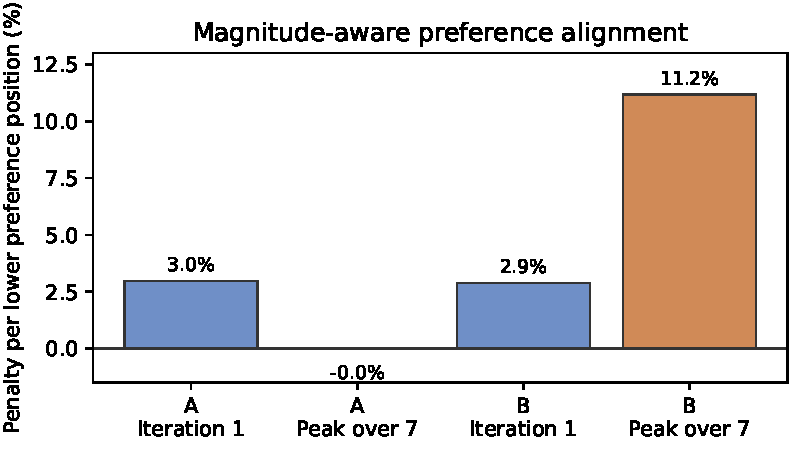
\includegraphics[width=\columnwidth]{preference_penalty.pdf}
  \caption{Rank-step penalty by prompt condition and horizon. Higher final
  penalty means Claude's ranking better predicts which starting direction
  reaches the best speedup after the fixed optimization budget.}
  \label{fig:penalty}
\end{figure}

\begin{table}[t]
\centering
\caption{Magnitude-aware alignment of agent ranking with speedup. Penalty is
percent lower speedup per one-step lower ranking position.}
\label{tab:penalty}
\scriptsize
\begin{tabular}{lrrr}
\toprule
\textbf{Condition} & \textbf{Iter. 1} & \textbf{Final} &
\textbf{Greedy} \\
\midrule
A default & 3.0\% & 0.0\% & +3.0 pp \\
B long-horizon & 2.9\% & 11.2\% & -8.3 pp \\
\bottomrule
\end{tabular}
\end{table}

The long-horizon prompt changes what the ranking predicts. Its iteration-1
penalty remains similar at 2.9\%, but its final-speedup penalty rises to
11.2\% per lower ranking position. The greediness score flips from +3.0
percentage points to -8.3 percentage points: the ranking becomes more aligned
with final speedup than with first-step payoff. This is the cleanest evidence
that the prompt does not simply make every branch faster. It changes Claude's
preference over starting directions.

\subsection{Practical Regret from Trusting P1}

Figure~\ref{fig:regret} and Table~\ref{tab:regret} give the practical version
of the result. If a user follows Claude's first-ranked plan under the default
prompt, the average final-speedup regret is 26.1\%. With long-horizon
prompting, this drops to 10.8\%. The risk remains, but the cost of trusting the
first direction is substantially smaller.

\begin{figure}[t]
  \centering
  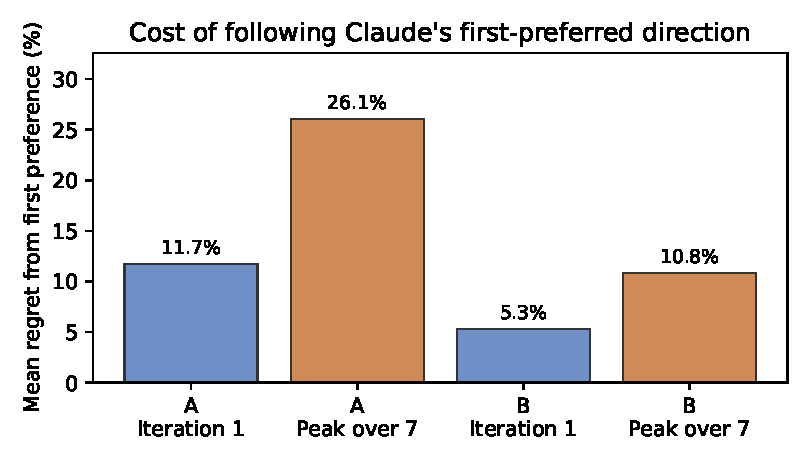
\includegraphics[width=\columnwidth]{top_choice_regret.pdf}
  \caption{Top-choice regret from following P1 instead of the best of P1--P5.
  The long-horizon prompt reduces regret at both horizons, especially for the
  final speedup found after the fixed Worker budget.}
  \label{fig:regret}
\end{figure}

\begin{table}[t]
\centering
\caption{Top-choice regret: speedup left on the table by following P1 instead
of the best of P1--P5.}
\label{tab:regret}
\scriptsize
\begin{tabular}{lrr}
\toprule
\textbf{Condition} & \textbf{Iter. 1 regret} & \textbf{Final regret} \\
\midrule
A default & 11.7\% & 26.1\% \\
B long-horizon & 5.3\% & 10.8\% \\
\bottomrule
\end{tabular}
\end{table}

The per-kernel regret values clarify where the average comes from. In the
default condition, P1 leaves 41.6\% final-speedup regret on bitonic-sort,
36.2\% on histogram, and 25.1\% on stencil3d, while softmax has only 1.5\%
regret. Therefore the default prompt's cost is not uniform. Its main failure is
that it sometimes misses the large-headroom direction, and pure ordering
metrics would not distinguish those costly misses from the small softmax near
tie.

\subsection{Raw Outcome Pattern}

Table~\ref{tab:rawpeak} shows the best speedup found by each ranked plan. It
makes the aggregate metrics inspectable: Condition A never has P1 as the
final-speedup winner, while Condition B has P1 winners for bitonic-sort and
stencil3d. Histogram B remains imperfect because P2 wins strongly. Softmax is
the important magnitude lesson: P5 wins in both conditions, but the performance
cluster is comparatively tight, especially in Condition A.

\begin{table*}[t]
\centering
\caption{Best speedup within the fixed Worker budget by agent-ranking
position. P1 is Claude's first-ranked plan.}
\label{tab:rawpeak}
\scriptsize
\begin{tabular}{llrrrrrc}
\toprule
\textbf{Kernel} & \textbf{Cond.} & \textbf{P1} & \textbf{P2} &
\textbf{P3} & \textbf{P4} & \textbf{P5} & \textbf{Winner} \\
\midrule
bitonic-sort & A & 1.382 & 1.409 & 2.366 & 1.001 & 1.000 & P3 \\
histogram    & A & 0.971 & 1.521 & 1.014 & 1.052 & 1.519 & P2 \\
softmax      & A & 1.653 & 1.620 & 1.656 & 1.619 & 1.677 & P5 \\
stencil3d    & A & 2.198 & 2.204 & 2.932 & 2.751 & 2.318 & P3 \\
bitonic-sort & B & 1.915 & 1.449 & 1.529 & 1.702 & 1.118 & P1 \\
histogram    & B & 1.464 & 2.286 & 1.002 & 1.002 & 1.025 & P2 \\
softmax      & B & 1.438 & 1.512 & 1.482 & 1.513 & 1.553 & P5 \\
stencil3d    & B & 4.985 & 2.296 & 2.298 & 1.476 & 2.778 & P1 \\
\bottomrule
\end{tabular}
\end{table*}

\subsection{Trajectory Evidence}

Figure~\ref{fig:traj} shows representative trajectories. Bitonic-sort A shows
an immediate-win plateau: P1 starts and ends at 1.382$\times$, while P3 starts
near baseline and later reaches 2.366$\times$. Histogram B shows the opposite:
P2 starts at 0.599$\times$ because the first implementation has too few
blocks, but recovers to 2.286$\times$ after grid tuning. Stencil3d B shows the
positive case for long-horizon prompting, where P1 moves from 2.927$\times$ to
4.623$\times$ to 4.985$\times$ through a coherent dependency chain.

\begin{figure}[t]
  \centering
  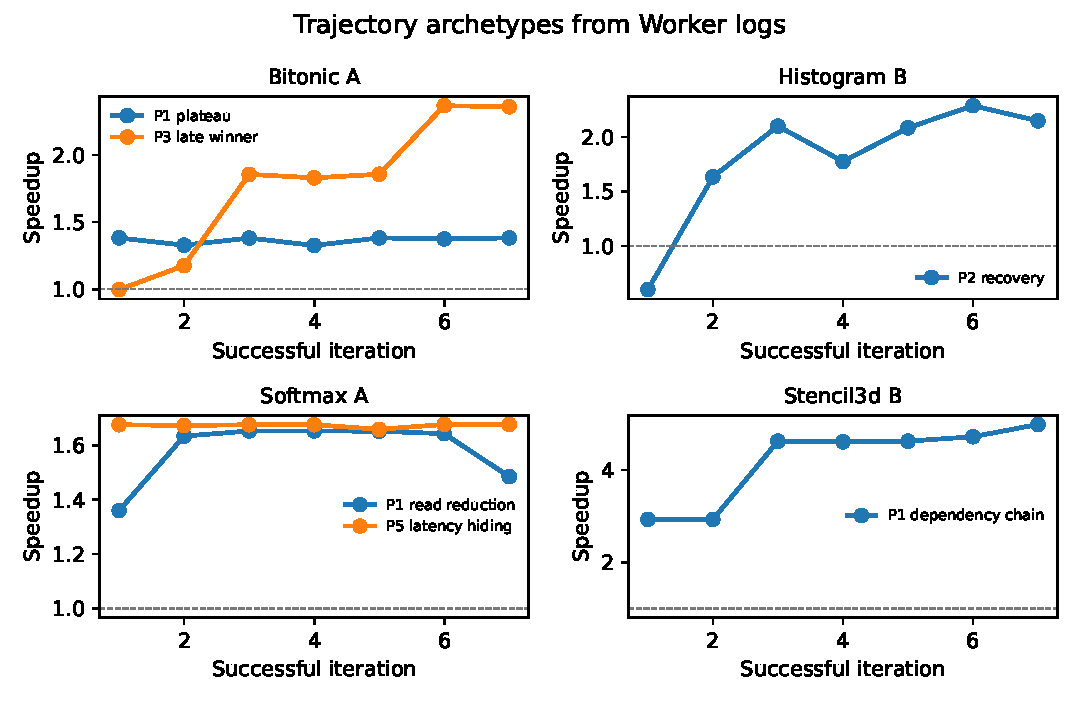
\includegraphics[width=\columnwidth]{trajectory_cases.pdf}
  \caption{Representative Worker trajectories. First-iteration speedup can
  overstate or understate the value of the starting direction.}
  \label{fig:traj}
\end{figure}

\subsection{Headroom After the First Step}

Table~\ref{tab:headroom} summarizes the same point numerically. Histogram B
P2 is the most extreme case: the first successful implementation is only
0.599$\times$, but the branch later reaches 2.286$\times$, a 3.82$\times$
recovery. Bitonic A P3 similarly starts near baseline and later wins. In
contrast, Bitonic A P1 has no headroom after its quick first win. These cases
show why evaluating only the next benchmark run would reward the wrong
behavior for this task.

\begin{table}[t]
\centering
\caption{Headroom after the first successful iteration.}
\label{tab:headroom}
\scriptsize
\begin{tabular}{lcrrr}
\toprule
\textbf{Case} & \textbf{P} & \textbf{First} & \textbf{Peak} &
\textbf{Recovery} \\
\midrule
Histogram B & P2 & 0.599 & 2.286 & 3.82$\times$ \\
Bitonic A & P3 & 0.997 & 2.366 & 2.37$\times$ \\
Histogram A & P5 & 0.656 & 1.519 & 2.32$\times$ \\
Stencil3d B & P1 & 2.927 & 4.985 & 1.70$\times$ \\
Bitonic A & P1 & 1.382 & 1.382 & 1.00$\times$ \\
\bottomrule
\end{tabular}
\end{table}

\section{Discussion and Root-Cause Analysis}

\subsection{Failures Are Structured}

The quantitative pattern is not random. Table~\ref{tab:taxonomy} summarizes
the main log-derived cases. These cases explain why the default ranking can
look reasonable in the first iteration while failing to identify the best
trajectory. They also show why the long-horizon prompt helps only sometimes:
Claude must still choose the correct causal mechanism.

\begin{table*}[t]
\centering
\caption{Root-cause taxonomy from Worker logs.}
\label{tab:taxonomy}
\scriptsize
\begin{tabular}{p{0.14\textwidth}p{0.22\textwidth}p{0.26\textwidth}p{0.28\textwidth}}
\toprule
\textbf{Case} & \textbf{Trajectory} & \textbf{Reasoning category} &
\textbf{Lesson} \\
\midrule
Bitonic A & Immediate plateau vs. slow-start winner &
Under-valued structural headroom &
First-step speedup can hide limited headroom. \\
Histogram B & Bad first implementation recovers &
Productive recovery &
Do not prune solely on the first attempt. \\
Softmax A/B & Close outcomes, wrong mechanism &
Correct bottleneck but wrong lever; elegance bias &
Need causal mechanism selection, not only profiler awareness. \\
Stencil3d B & Dependency-chain success &
Correct direction and mechanism &
Long-horizon prompting helps when later moves build on the first. \\
\bottomrule
\end{tabular}
\end{table*}

In bitonic-sort A, P1 fused shared-memory stages and immediately achieved
1.382$\times$, but logs reported significant shared-memory bank conflicts and
increased registers per thread. The branch never improved beyond that. P3
began with a host-side cleanup that did almost nothing, 0.997$\times$, but
later found the real structural path: shared-memory efficiency, linear
thread-to-comparison mapping, and reduced divergence. It peaked at
2.366$\times$. This is the clearest example of why first-step speedup is a
weak proxy for trajectory value: the quick win addressed visible memory
behavior but left little headroom.

Histogram B shows the complementary risk. P2 initially slowed to
0.599$\times$ because the first single-pass implementation used too few blocks
for a 1920-by-1080 image. The strategy itself was strong: it removed a second
kernel launch and a global write/read round trip. After grid sizing restored
parallelism and balanced atomic contention, the branch reached 2.286$\times$.
A strict ``must improve immediately'' policy would have discarded one of the
best directions. This is directly relevant to agent search design: early
failure can be an implementation parameter error rather than a bad hypothesis.

\subsection{Profiling-Aware Is Not Causal}

Softmax is the key reasoning-quality counterexample. In Condition A, Claude
noticed memory behavior and ranked read-reduction plans highly. P1 reduced
global reads from three passes to one and halved exponential calls, but
occupancy fell from 74.1\% to 30.7\%. P5, a lower-ranked block-per-slice
direction, won by increasing per-slice parallelism: occupancy rose to 94.7\%
and memory stalls fell from 94.5\% to 60.1\%. The practical regret was small in
Softmax A because outcomes were close, but the mechanism lesson is important:
the stronger lever was latency hiding, not simply reducing memory traffic.

Condition B backfired differently. Claude ranked online softmax first, an
algorithmically elegant rewrite that reduced a global read pass. It peaked at
1.438$\times$. The fifth-ranked branch, simple block-size tuning, reached
1.553$\times$ by improving scheduler utilization. The long-horizon prompt
encouraged a sophisticated algorithmic story, but the hardware bottleneck
favored a simpler launch-configuration knob. Thus access to profiling evidence
is not enough; the agent needs causal resource accounting: which metric is the
bottleneck, which is a symptom, and what cost another resource pays.

\subsection{When Long-Horizon Prompting Helps}

Stencil3d B shows the success case. Claude ranked double-to-float first. The
first step halved memory traffic and raised occupancy, reaching
2.927$\times$. The Worker then used profiler evidence to adjust block shape,
raising global load efficiency and speedup to 4.623$\times$, and later tuned
XTILE to reach 4.985$\times$. The first move was valuable because it unlocked
later coalescing and tiling improvements. This suggests that long-horizon
prompting helps most when the dependency chain between first edit and later
optimizations is visible.

The contrast with softmax is important. Both kernels are memory-related, but
only stencil3d offered an obvious chain where one foundational resource change
made later optimization easier. In softmax, several plausible mechanisms
competed: fewer reads, more occupancy, more outstanding work, and launch
configuration. The long-horizon prompt could not by itself decide which
mechanism had causal leverage. This points to a design implication: prompting
should be paired with tools that force the agent to maintain a bottleneck
hypothesis ledger and account for resource tradeoffs.

\subsection{Implications for Agent Design}

The results suggest three concrete requirements for LLM-based kernel
optimization systems. First, the system should preserve multiple hypotheses
instead of committing to the first fast improvement. Histogram B P2 would be
lost under a strict first-step-improvement filter, even though it becomes the
best histogram trajectory. Second, the system should evaluate magnitude, not
only order. Softmax A is an ordering miss, but its regret is small; bitonic A
and histogram A are the cases where the first choice is actually costly.
Third, the agent needs structured causal accounting over GPU resources. A useful
debugging trace should record the current bottleneck hypothesis, the expected
resource tradeoff, the observed profiler change, and whether the evidence
supports or contradicts the hypothesis. That is the missing layer between
having profiler data and using it correctly.

\subsection{Threats to Validity}

The study is small: four kernels and five generated plans per condition. The
statistics are descriptive rather than significance claims. Worker quality also
affects measured trajectory value; a branch may underperform because the Worker
did not find the best implementation of its assigned plan within the budget.
This is partly intentional, because the experiment evaluates a realistic
plan-generation plus Worker workflow rather than oracle implementations.
Finally, results may vary with GPU architecture, prompt wording, and benchmark
choice. The value of the study is as a controlled diagnostic of Claude's
optimization preference, not as a broad claim about all kernels or all LLMs.

\section{Conclusion}

Claude's default first-move preference is mildly aligned with immediate
speedup but weakly aligned with the best speedup found after continuing
optimization. Explicit long-horizon prompting changes this behavior: the
ranking becomes more predictive of final speedup and top-choice regret falls
from 26.1\% to 10.8\%. Prompting alone is not enough. The logs reveal recurring
causal failures around salient metrics, mechanism selection, algorithmic
elegance, and resource tradeoffs. The practical lesson is to treat Claude's
first plan as a hypothesis, not a decision: robust LLM optimization systems
should preserve multiple hypotheses, evaluate trajectory value, and provide
structured tools for causal GPU-resource accounting.

\begin{thebibliography}{00}
\bibitem{hecbench}
Z. Jin, ``HecBench: Heterogeneous Computing Benchmark Suite,'' GitHub
repository. [Online]. Available:
\url{https://github.com/zjin-lcf/HeCBench}

\bibitem{cuda}
NVIDIA, ``CUDA C++ Programming Guide.'' [Online]. Available:
\url{https://docs.nvidia.com/cuda/cuda-c-programming-guide/}

\bibitem{ncu}
NVIDIA, ``Nsight Compute User Guide.'' [Online]. Available:
\url{https://docs.nvidia.com/nsight-compute/}

\bibitem{claude}
Anthropic, ``Claude Code.'' [Online]. Available:
\url{https://www.anthropic.com/claude-code}
\end{thebibliography}

\clearpage
\xdef\mainbodyendpage{\thepage}

\appendices

\section{Input Prompts}

The human prompt to the plan-generating Claude session was intentionally short;
the generated condition README contained the full task, source code, profiling
digest, and output contract.

\begin{lstlisting}
Read README.md and write response.json exactly as instructed.
\end{lstlisting}

The human prompt to each Worker branch was:

\begin{lstlisting}
Read README.md and strictly follow it.
\end{lstlisting}

Full prompt surfaces are documented in:

\begin{lstlisting}
README.md
EXPERIMENT_PLAN.md
experiments/<kernel>/cond_<A|B>/README.md
experiments/<kernel>/cond_<A|B>/workers/branch_<rank>/README.md
\end{lstlisting}

\section{System Prompt and Agent Instructions}

The experiment did not rely on a separate hidden prompt authored during the
experiment. The controlled agent instruction surface was the generated Planner
and Worker README text. The role instructions embedded in those files are
excerpted below.

Planner role instruction:
\begin{lstlisting}
You are a CUDA optimization expert.
\end{lstlisting}

Worker role instruction:
\begin{lstlisting}
You are the Worker agent. Optimize this kernel according to the assigned plan below.
\end{lstlisting}

The Worker README also instructed the agent to stay in its branch directory,
edit only allowlisted source files, run \texttt{./src/run.sh} after each edit,
treat failed attempts as non-counting, and maintain \texttt{LOG.md}.

\section{Prompt Condition Excerpts}

Condition A opening:
\begin{lstlisting}
# CUDA Kernel Optimization Request: <kernel>

You are a CUDA optimization expert. The user wants to optimize the CUDA kernel below.

Propose exactly five distinct optimization plans and rank them from highest to lowest priority based on what you would try first to improve this kernel's performance.
\end{lstlisting}

Condition B opening:
\begin{lstlisting}
# CUDA Kernel Optimization Request: <kernel>

You are a CUDA optimization expert. A separate Claude Code Worker will execute each ranked plan for exactly 7 iterations.

Propose exactly five distinct optimization plans and rank them by which starting direction is most likely to achieve the highest peak speedup at any point within those 7 iterations. Consider how the first direction opens or blocks later optimizations.
\end{lstlisting}

Shared output contract:
\begin{lstlisting}
Write your answer to exactly this file:

response.json

response.json must be a JSON array of exactly five objects. Each object may contain only these two fields:
- rank
- plan
\end{lstlisting}

\section{Representative Agent Output}

Softmax Condition B P1, representative plan:
\begin{lstlisting}
{
  "rank": 1,
  "plan": "Implement online (single-pass) softmax to eliminate one full global read pass, combined with float4 vectorized loads. Currently softMax2 makes 3 separate warp-strided passes over global memory ... Target bottleneck: the 3x global memory read passes ... reducing to 2 passes ... Correctness risk: the online rescaling formula ..."
}
\end{lstlisting}

\section{Changes Made to the Agent Workflow}

The experiment used a generated Planner/Worker harness rather than a single
continuous agent session. The key workflow changes were:

\begin{itemize}
\item Planner/Worker split, so plan preference is measured before implementation
outcomes are known.
\item Two plan-generation prompts: default priority ordering and explicit
long-horizon trajectory ordering.
\item Five isolated Worker branches per condition.
\item Seven-successful-iteration rule; failed attempts are logged but do not
count toward the budget.
\item Correctness gate before timing contributes to analysis.
\item Fixed JSON contracts for \texttt{response.json}, per-run
\texttt{run.json}, and condition-level \texttt{analysis.json}.
\item Worker source-edit allowlist and protected-file checks.
\item Reproducible artifact generation through the report artifact script.
\end{itemize}

Architecture and file-format details are documented in:
\begin{lstlisting}
README.md
EXPERIMENT_PLAN.md
\end{lstlisting}

\section{Additional Results Tables}
\FloatBarrier

\begin{table}[H]
\centering
\caption{Per-kernel final-speedup regret from following P1.}
\scriptsize
\begin{tabular}{lccrr}
\toprule
\textbf{Kernel} & \textbf{Cond.} & \textbf{Winner} & \textbf{P1} &
\textbf{Regret} \\
\midrule
bitonic & A & P3 & 1.382 & 41.6\% \\
histogram & A & P2 & 0.971 & 36.2\% \\
softmax & A & P5 & 1.653 & 1.5\% \\
stencil3d & A & P3 & 2.198 & 25.1\% \\
bitonic & B & P1 & 1.915 & 0.0\% \\
histogram & B & P2 & 1.464 & 35.9\% \\
softmax & B & P5 & 1.438 & 7.4\% \\
stencil3d & B & P1 & 4.985 & 0.0\% \\
\bottomrule
\end{tabular}
\end{table}

\section{Representative Log Evidence}
\FloatBarrier

\begin{table*}[!htbp]
\centering
\caption{Short log excerpts used for root-cause analysis.}
\scriptsize
\begin{tabular}{p{0.20\textwidth}p{0.36\textwidth}p{0.34\textwidth}}
\toprule
\textbf{Claim} & \textbf{Source} & \textbf{Excerpt} \\
\midrule
Bitonic A P1 plateau &
\texttt{.../bitonic-sort-cuda/cond\_A/branch\_1/LOG.md} &
``Fusing smem stages gives 1.38x speedup... significant smem bank conflicts...
Registers/thread increased to 39.'' \\
Bitonic A P3 recovery &
\texttt{.../bitonic-sort-cuda/cond\_A/branch\_3/LOG.md} &
``Global load efficiency improved to 100\%, occupancy to 92.4\%. Shared memory
approach is the right direction.'' \\
Histogram B P2 first failure &
\texttt{.../histogram-cuda/cond\_B/branch\_2/LOG.md} &
``64 blocks is not enough to cover the 1920x1080 image efficiently...
serializing work.'' \\
Softmax A mechanism miss &
\texttt{.../softmax-cuda/cond\_A/branch\_1/LOG.md} &
``Smem reduced global loads from 3x to 1x and halved expf, but occupancy
dropped from 74.1\% to 30.7\%.'' \\
Softmax B simple winner &
\texttt{.../softmax-cuda/cond\_B/branch\_5/LOG.md} &
``BLOCK\_SIZE=512 improved from 1.48x to 1.55x. More warps per SM improves
scheduler utilization.'' \\
Stencil3d B chain &
\texttt{.../stencil3d-cuda/cond\_B/branch\_1/LOG.md} &
``Float halved memory traffic and boosted occupancy from 79.6\% to 96.7\%.'' \\
\bottomrule
\end{tabular}
\end{table*}
\FloatBarrier

Complete evidence indices are included in:
\begin{lstlisting}
analysis/evidence/case_evidence_index.md
analysis/evidence/log_taxonomy.csv
\end{lstlisting}

\section{Analysis Artifacts}

The final report numbers come from:
\begin{lstlisting}
analysis/data/metric_summary.csv
analysis/data/greediness_summary.csv
analysis/data/top_choice_regret_summary.csv
analysis/data/top_choice_regret_by_kernel.csv
analysis/data/peak_speedup_by_preference.csv
analysis/data/headroom_recovery.csv
analysis/notes/results_summary.md
\end{lstlisting}

\end{document}
